\documentclass[a4paper]{extreport}
\usepackage[14pt]{extsizes}
\usepackage{cmap}
\usepackage[T2A]{fontenc}
\usepackage[utf8]{inputenc}
\usepackage[english,russian]{babel}
\usepackage{amsmath}
\usepackage{amsfonts}
\usepackage{graphicx}
\usepackage{algorithm}
\usepackage{algpseudocode}
\usepackage[a4paper,nofoot,left=30mm,right=10mm,top=20mm,bottom=20mm]{geometry}
\usepackage{hyperref}
\linespread{1.3}
\usepackage{indentfirst}
\newcommand{\angstrom}{\text\normalfont\AA}
\newcommand{\bb}{\textbf}
\newcommand{\ls}{\left[}
\newcommand{\rs}{\right]}
\newcommand{\lp}{\left(}
\newcommand{\rp}{\right)}
\newcommand{\la}{\leftarrow}
\newcommand{\eps}{\varepsilon}
\begin{document}
\begin{titlepage}
\begin{center}
    \small
    \textbf{МИНИСТЕРСТВО ОБРАЗОВАНИЯ РЕСПУБЛИКИ БЕЛАРУСЬ}
    \vspace{0.25cm}
    \textbf{БЕЛОРУССКИЙ ГОСУДАРСТВЕННЫЙ УНИВЕРСИТЕТ}
    \vspace{0.25cm}
    \textbf{ФАКУЛЬТЕТ ПРИКЛАДНОЙ МАТЕМАТИКИ И ИНФОРМАТИКИ}
    \vspace{0.25cm}
    \normalsize
    \textbf{Кафедра биомедицинской информатики}
    \vfill
        \large
    \textbf{Разработка среды для построения структур белковых комплексов}
    \vfill
    \normalsize
    Курсовая работа
\end{center}
\vfill
\hfill\begin{minipage}{0.5\textwidth}
    Рака Алексей Степановича\\
    студента 3 курса,\\
    специальность <<Информатика>>
    \vspace{0.25cm}
    \\
    Научный руководитель:\\
    Хадарович А.Ю.
\end{minipage}
\bigskip
\begin{center}
    Минск, 2018
\end{center}
\end{titlepage}
\tableofcontents
\newpage
\normalsize
\addcontentsline{toc}{chapter}{Введение}
\chapter*{ Введение }
Выравнивание структуры белка – это ценный инструмент для фолдинга белков и классифицикации функций. Успех структурной геномики, направленной на экспериментальное определение трёхмерных структур тысяч репрезентативных белков, в решающей степени зависит от нашей способности разрабатывать точные инструменты для сравнения белковых структур. Однако, несмотря на свою исключительную важность, проблема по-прежнему не имеет быстрого и точного решения. В то время, как некоторые функции скоринга структурного подобия могут быть аппроксимированы за полиномиальное время, нет никакой процедуры для оптимизации любой меры структурного выравнивания. В своей обзорной статье о прогрессе в области сравнения структур Тейлор и коллеги пишут: “в сравнении структур у нас даже нет алгоритма, который гарантирует оптимальный ответ для пары структур”.

Существует несколько различных, но связанных между собой определений оптимального выравнивания двух белков. Некоторые методы определяют оптимальную суперпозицию, минимизирующую расстояние между выровненными атомами. Другие методы пытаются минимизировать разницу между внутриатомными расстояниями.

Недавно было введено несколько методов улучшения соответствия белковых структур, включая методы, основанные на фенотипической пластичности и метод гибких выравниваний последовательностью локальных преобразований.

Пожалуй, наиболее интуитивной и широко используемой мерой подобия двух белков является наибольшее количество атомов в двух структурах, которые могут быть совмещены друг с другом на заданное расстояние. Далее будем обозначать эту матрицу $CA \leq \sigma$, где $\sigma > 0$ обозначает порог расстояния в ангстремах.

Многие меры структурного выравнивая построены на $CA \leq \sigma$, включая GDT, AL0, MaxSub, CA-atoms < 3\angstrom, Q-score и TM-score. Global Distance Test (GDT) обычно используется для оценки качества моделей в эксперименте CASP. Точность прогнозируемой модели в CASP измеряется оценкой GDT\_TS, которая представляет собой среднее значение оценок GDT, вычисленных на нескольких порогах расстояния. Точнее,
\begin{gather*}
\mathrm{GDT\_TS} = \frac{(\mathrm{GDT\_P1} + \mathrm{GDT\_P2} + \mathrm{GDT\_P4} + \mathrm{GDT\_P8})}{4}
\end{gather*}

Где $\mathrm{GDT\_Pn}$ определяет часть атомов CA, которые могут быть совмещены на расстоянии не превосходящем n ангстремов.

Одной из главных мер качества модели в LiveBench является CA-atoms < 3 \angstrom (в наших обозначениях CA < 3). Из-за сложности оптимизации самой функции подсчёта очков LiveBench приближается к CA < 3 с помощью 3deval, программы, которая пытается максимизировать другую матрицу, а именно 3D-оценку.

CAFASP бенчмарк использует MsxSub для оценки качества прогнозов. MaxSub определяется как взвешенная доля остатков в модели, попадающих в пределы 3.5 \angstrom от выровненных остатков в экспериментальной структуре.

Независимо от используемой системы подсчёта очков, основная трудность, которую должен преодолеть любой метод структурного выравнивания, -- это бесконечное (несчётное) пространство всех возможных структурных суперпозиций. Чтобы обойти эту проблему, текущие исследования в этой области фокусируются на уменьшении размера пространства поиска путём перечисления относительно небольшого, но репрезентативного набора суперпозиций. Однако, хотя решения, полученные эвристическими подходами, частично точны, они никогда не гарантируются даже близкими к оптимальным решениями.

Очевидным способом устранения ограничений эвристических методов является разработка быстрого и точного метода максимизации $CA \leq \sigma$. Такой метод позволил бы точно вычислить ряд мер структурного выравнивания, включая GDT\_TS, AL0 и MaxSum.

В данной работе рассмотрим алгоритм, который способен найти суперпозицию, которая достаточно близка к оптимальной суперпозиции. Более конкретно, для любого заданного расстояния среза $\sigma > 0$ и любого $\eps > 0$ алгоритм возвращает суперпозицию, которая помещает по крайней мере столько пар остатков на расстоянии не превосходящем $\sigma + \eps$ сколько оптимальная суперпозиция содержит пар на расстоянии не превосходящем $\sigma$. В дополнение к относительно низкой временной сложности и способности к параллельным реализациям, данный алгоритм обеспечивает "качество решения", которое определяется как разница между оценкой возвращённой суперпозиции и оценкой оптимальной суперпозиции. Метрика качества решения может использоваться для определения того, является ли возвращённая суперпозиция оптимальной суперпозицией (или необходим дургой более подробный поиск).

Данный алгоритм приближённого решения основан на схеме Колодного и Линиала для аппроксимации для класса непрерывных мер структурного подобия, работающей за полиномиальное время. Однако представленные здесь  результаты не могут быть получены из их исследования, поскольку целевая функция $CA \leq \sigma$ не относится к категории оценочных функций описываемых Колодным и Линиалом функций. На самом деле, класс оценочных функций поддающихся методам Колодного и Линиала (а именно в классу функций удовлетворяющих условию Липшица) не включает в себя GDT\_TS, AL0, MaxSum, TM-score, Q-score и некоторые другие меры структурного сходства белков.

Наконец, в данной работе решается проблема нахождения процедуры, которая возвращает оптимальную суперпозицию двух структур. Здесь представляется процедура, которая гарантированно вернёт оптимальное решение с вероятностью 1, т.е. для всех, кроме конечного значений, расстояний. Однако подчеркнём, что алгорим оптимального решения не работает за полиномиальное время. Так же известно, что это проблема является NP-трудной.

\chapter{Пространственное выравнивание белков}

Пространственное выравнивание — способ установления гомологии между двумя или более полимерными структурами на основании их трёхмерной структуры. Этот процесс обычно применяется к третичной структуре белков, но может также использоваться и для больших молекул РНК. В противоположность простому наложению структур, когда известно по крайней мере несколько эквивалентных аминокислотных остатков, пространственное выравнивание не требует никаких предварительных данных, кроме координат атомов.

Пространственное выравнивание подходит для сравнения белков с непохожими последовательностями, когда эволюционные отношения не могут быть установлены стандартными методами выравнивания последовательностей, но в этом случае необходимо принимать во внимание влияние конвергентной эволюции.

Пространственное выравнивание позволяет сравнивать две и более молекулы, для которых известны трехмерные структуры. Два основных метода их получения — рентгеноструктурный анализ и ЯМР-спектроскопия. Для пространственного выравнивания можно также использовать структуры, полученные методами предсказания структуры белка. Пространственные выравнивания особенно важны для анализа данных, полученных методами структурной геномики и протеомики, они также могут использоваться для оценки выравниваний, полученных путём сравнения последовательностей. 

\section{Данные, получаемые путём структурного выравнивания}

Результатом работы программ структурного выравнивания, как правило, является совмещение наборов координат атомов и наименьшее среднеквадратическое отклонение (RMSD) между структурами. Кроме того, могут быть рассчитаны и более сложные параметры, оценивающие структурное сходство, например, тест глобальных расстояний. RMSD указывает на степень расхождения выравниваемых структур. Структурное выравнивание может быть затруднено из-за наличия нескольких доменов в структуре выравниваемых белков, так как изменения в относительном расположении этих доменов между двумя структурами могут искусственно изменять значение RMSD. Из структурного выравнивания непосредственно вытекает соответствующее одномерное выравнивание последовательностей, кроме того, на его основании можно рассчитать долю аминокислотных остатков, идентичных между двумя белками. 

\section{Типы сравнений}

Для создания структурного выравнивания и подсчёта соответствующих значений RMSD могут быть использованы как все атомы, входящие в молекулу белка, так и их подмножества. Например, атомы боковых радикалов аминокислотных остатков учитываются не всегда, и для выравнивания могут использоваться только атомы, входящие в пептидный остов молекулы. Такой вариант выбирают, если у выравниваемых структур очень разная аминокислотная последовательность и боковые радикалы различаются у большого числа остатков. По этой причине по умолчанию методы пространственного выравнивания используют только атомы остова, вовлечённые в пептидную связь. Для большего упрощения и увеличения эффективности часто используется положение только альфа-атомов углерода, так как их положение достаточно точно определяет положение атомов полипептидного остова. Только при выравнивании очень похожих или даже идентичных структур важно учитывать позиции атомов боковых цепей. В этом случае RMSD отражает не только схожесть конформации белкового остова, но и ротамерные состояния боковых цепей. Другие способы, позволяющие снизить шум и увеличить число правильных сопоставлений, используют разметку элементов вторичной структуры, карты нативных контактов или паттерны взаимодействия остатков, меры степени упаковки боковых цепей и меры сохранения водородных связей.

Самый простой способ сравнить две структуры не требует выравнивания самих структур, а использует выравнивание последовательностей. Оно определяет, какие пары аминокислотных остатков сопоставлены друг другу, и затем только они используются для подсчёта RMSD. Наложение структур обычно используется для сравнения нескольких конформаций одного белка (в этом случае даже не нужно выравнивать последовательности) и для оценки качества выравниваний последовательностей, если для них известны структуры. Традиционно при наложении структур используется простой метод наименьших квадратов, в котором оптимальные повороты и трансляции находят через минимизацию суммы квадратов расстояний между всеми структурами в наложении. В недавнее время подобный поиск стал более точным благодаря методам максимального правдоподобия и байесовским методам.

Алгоритмы, основанные на многомерных поворотах и модифицированных кватернионах, были разработаны для определения топологических отношений между структурами белков без построения выравнивания последовательностей. Такие алгоритмы успешно определили канонические укладки, такие как четырёхспиральный пучок. Метод SuperPose позволяет учитывать относительные вращения доменов и другие сложные моменты структурного выравнивания.

\section{Представление структур}

Для того чтобы сравнивать структуры белков, нужно представить их в пространстве, которое не зависит от координат. Это обычно достигается с помощью матрицы «последовательность против последовательности» или серии матриц, которые включают меры сравнения, относящиеся к фиксированному пространству координат, а не абсолютные расстояния. Очевидным способом подобного представления является матрица расстояний, которая представляет собой двумерную матрицу, содержащую все попарные расстояния между некоторым набором атомов в каждой структуре (например, альфа-атомами углерода). Размерность такой матрицы с увеличением числа одновременно сравниваемых структур растёт. Представив белок в виде крупных частей, таких как элементы вторичной структуры (SSEs) или другие структурные фрагменты, тоже можно получить разумное выравнивание, несмотря на потерю информации от неучтенных расстояний, так как не будет учитываться и шум от них. Таким образом, выбор способа представления белка для облегчения вычислений является критическим для разработки эффективного алгоритма выравнивания.  

\section{Вычислительная сложность}

Оптимальное решение

Было показано, что оптимальное «протягивание» белковой последовательности через известную структуру и построение оптимального множественного выравнивания последовательностей являются NP-полными задачами. Однако обычная задача структурного выравнивания не является NP-полной. Строго говоря, оптимальное решение задачи структурного выравнивания белков известно только для некоторых мер сходства белковых структур -- например, мер, используемых в задачах предсказания структуры белка GDT\_TS и MaxSub. Такие меры могут быть оптимизированы, используя алгоритм, способный максимизировать число атомов в двух белках, которые могут быть совмещены, так как удовлетворяют предустановленному порогу на расстояние между ними. К сожалению, алгоритм оптимального выравнивания непрактичен, так как время его работы зависит не только от длин последовательностей, но и от геометрии выравниваемых белков.

Приближенное решение

Были разработаны и приближённые алгоритмы структурного выравнивания, работающие полиномиальное время и выдающие целое семейство «оптимальных» решений в пределах параметра приближения для заданной функции счёта. Хотя теоретически задача приближённого структурного выравнивания белков легко даётся таким алгоритмам, они всё равно являются вычислительно затратными для масштабного анализа белковых структур. Как следствие, не существует практичных алгоритмов, которые с заданной функцией счёта сходились бы к глобальному решению выравнивания. По этой причине большинство алгоритмов являются эвристическими, но всё же были разработаны практичные алгоритмы, которые гарантируют схождение хотя бы к локальной максимизации функции счёта. 

\section{Методы}

Структурное выравнивание используется как при сравнении отдельных структур или их наборов, так и при создании баз данных сравнений «все-против-всех» («all-to-all»), которые отражают различия между каждой парой структур, присутствующих в Protein Data Bank (PDB). Такие базы данных обычно используются для классификации белков по их укладке.

DALI

Одним из популярных методов структурного выравнивания является DALI (англ. distance alignment matrix method — метод с использованием матрицы дистанционных выравниваний). В нём исходные структуры белков разбиваются на гексапептиды и через оценку паттернов контактов между фрагментами рассчитывается матрица расстояний. Элементы вторичной структуры, остатки которых являются соседними в последовательности, оказываются на главной диагонали матрицы; остальные диагонали матрицы отражают пространственные контакты между остатками, которые в последовательности не находятся рядом друг с другом. Если эти диагонали параллельны главной диагонали, то элементы вторичной структуры, которые они представляют, тоже параллельны; если они, напротив, перпендикулярны ей, то их элементы вторичной структуры антипараллельны. Такое представление интенсивно работает с памятью, так как используемая матрица симметрична относительно главной диагонали (и потому избыточна).

Когда матрицы расстояний двух белков имеют одинаковые или похожие элементы примерно на одинаковых позициях, можно сказать, что белки имеют схожую укладку и их элементы вторичной структуры соединены петлями примерно одинаковой длины. Непосредственный процесс выравнивания DALI заключается в поиске схожестей матриц, построенных для двух белков; обычно это осуществляется с помощью серии перекрывающихся подматриц размера 6 $\times$ 6. Соответствия подматриц потом пересобираются в конечное выравнивание с помощью стандартного алгоритма максимизации счёта. Оригинальная версия DALI использует симуляцию Монте-Карло для максимизации значения пространственной схожести, являющегося функцией от расстояний между предполагаемыми соответствующими атомами. В частности, вес более отдалённых атомов внутри соответствующих элементов структуры экспоненциально занижается, чтобы уменьшить шум, вызванный подвижностью петель, искривлением спиралей и другими мелкими вариациями структур. Поскольку DALI основан на матрице расстояний типа «все-против-всех», метод может учитывать расположение элементов структур в различном порядке в двух сравниваемых последовательностях.

Метод DALI был использован для создания базы данных FSSP (англ. Families of Structurally Similar Proteins), в которой все известные структуры белков были попарно выровнены для определения их пространственного родства и классификации укладок.

DaliLite является скачиваемой программой, использующей алгоритм DALI.

Комбинаторное расширение

Метод комбинаторного расширения (англ. Combinational extension (СЕ)) похож на DALI тем, что тоже разбивает каждую структуру на ряд фрагментов, которые затем пытается заново собрать в полное выравнивание. Серия попарных сочетаний фрагментов, называемых AFP (англ. aligned fragment pairs — пары выровненных фрагментов), используется для задания матрицы сходства, через которую прокладывается оптимальный путь для определения конечного выравнивания. Только те AFP, которые удовлетворяют заданным критериям локального сходства, включаются в матрицу, что сокращает необходимое пространство поиска и увеличивает эффективность. Возможны разные меры сходства; в первоначальном виде метод CE использовал только структурные совмещения и расстояния между остатками, но со временем был расширен для использования локальных свойств, таких как вторичная структура, доступность растворителя, паттерны водородных связей и двугранные углы.

Путь, соответствующий выравниванию, рассчитывается как оптимальный путь через матрицу сходства с помощью линейного прохода через последовательности, расширяя выравнивание следующей возможной AFP с высоким счётом. Начальная AFP, инициирующая выравнивание, может быть выбрана в любой точке матрицы последовательностей. Далее происходит расширение на AFP, которая удовлетворяет заданному критерию на расстояние, ограничивающему размер гэпов (разрывов) в выравнивании. Размер каждой AFP и наибольшая длина гэпа являются необходимыми входными параметрами, но обычно устанавливаются равными эмпирически определённым значениям 8 и 30 соответственно. Подобно DALI или SSAP, CE использовался для создания базы данных классификации укладок на основе известных пространственных структур белков из PDB. Недавно PDB выпустил обновлённую версию CE, которая может определять циклические перестановки в структуре белков.

SSAP

Метод SSAP (англ. Sequential Structure Alignment Program) использует двойное динамическое программирование для построения структурного выравнивания, основанного на векторах «от атома к атому» в пространстве структур. Вместо альфа-атомов углерода, обычно используемых в структурных выравниваниях, SSAP задаёт свои вектора из бета-атомов для всех аминокислотных остатков за исключением глицина. Таким образом, этот метод учитывает положение ротамера каждого остатка, также как и их положение в остове. Сначала SSAP для каждого белка строит серию векторов расстояний между каждым остатком и его ближайшим, но не смежным в последовательности соседом. После этого конструируется ряд матриц, содержащих разницу векторов между соседями для каждой пары остатков, для которых строились вектора. Для каждой получившейся матрицы с помощью динамического программирования определяется ряд оптимальных локальных выравниваний. Затем полученные выравнивания складываются в обобщённую матрицу, к которой снова применяется динамическое программирование для определения полного структурного выравнивания. Изначально SSAP создавал только попарные выравнивания, но в дальнейшем был расширен и для создания множественных выравниваний. Он был применён для выравнивания типа «все-против-всех» для создания иерархической системы классификации укладок, известной как CATH, которая используется в базе данных CATH Protein Structure Classification. 

\chapter{ Методы и результаты }

\section{Предварительные сведения и определения}

Задача выравнивания структуры пары белков может быть сформулирована следующим образом: "Учитывая два белка a и b и расстояние среза $\sigma > 0$, найти жёсткое преобразование $t$ и соответствие остаток-остаток (выравнивание), которое максимизирует количество пар остатков $a$ и $t(b)$ на расстоянии $\leq \sigma$". Мы называем $t$ -- $\sigma$-оптимальное преобразование для $a$ и $b$. Отметим, что, не теряя общности, можно предположить, что белок $a$ удерживается фиксированным, в то время как белок $b$ трансформируется.

Для того, чтобы точно сформулировать вышеуказанную проблему, нам нужны некоторые определения.

\bb{Определение} Белок -- это последовательность точек в трёхмерном пространстве:
\begin{gather*}
a = (a_1, a_2, \dots, a_n), a_i \in \mathbb{R}^3, i = \overline{1, n}
\end{gather*}

Во многих приложениях, $ a_i$ представляет собой CA-остаток.
\bb{Определение} Выравнивание белков $a = (a_1, a_2, \dots, a_n)$ и $b = (b_1, b_2, \dots, b_m)$ -- это последовательность пар точек из $a$ и $b$:
\begin{gather*}
S(a, b) = ((a_{i_1}, b_{j_1}), \dots, (a_{i_k}, b_{j_k}))
\end{gather*}
где $1 \leq i_1 < \dots < i_k \leq n$ и $1 \leq j_1 < \dots < j_k \leq m$.
\bb{Определение} $\sigma$-оптимальное выравнивание белков $a = (a_2, a_2, \dots, a_n)$ и $b = (b_1, b_2, \dots, b_m)$, обозначается $S(a, b, \sigma)$ это выравнивание $a$ и $b$, которое максимизирует число выровненных точек $a$ и $b$ на расстоянии $\sigma$.

В приведённом выше определении мы предполагаем, что белки $a$ и $b$ зафиксированы в пространстве. $S(a, b, \sigma )$ относятся к оптимальному спариванию аминокислотных букв буще изменения структурной суперпозиции. Хорошо известно, что для любых двух фиксированных в пространстве белков $a$ и $b$ длины $n$ и любого $\sigma > 0$  выравнивание $S(a, b, \sigma )$ может быть вычислено за время $O(n^2)$ с использованием динамического программирования. Теперь мы будем использовать $|S(a, b, \sigma )|$ для обозначения количества пар точек в $S(a, b, \sigma )$ на расстоянии $\leq \sigma$

\bb{Определение} $\sigma$-оптимальная трансформация для $a$ и $b$, обозначается $t^\sigma$, -- это жёсткая трансформация, которая максимизирует $|S(a, t(b), \sigma)|$ в множестве всех жёстких трансформаций. Другими словами:
\begin{gather*}
t^\sigma = \arg \max_t |S(a, t(b), \sigma)|
\end{gather*}

Легко увидеть, что CA $\leq \sigma$ в точность $|S(a, t^\sigma (b), \sigma)|$, где $t^\sigma$ -- это $\sigma$-оптимальная трансформация $a$ и $b$.

\bb{Определение} Трансформация $t$ удовлетворяет:
\begin{gather*}
|S(a, t(b), \sigma + \eps)| \geq |S(a, t^\sigma (b), \sigma)|
\end{gather*}

Это называется $(\sigma, \eps)$-трансформация $a$ и $b$, обозначается $t_\eps^\sigma$.

Нужно отметить, что $t_\eps^\sigma$ -- это любая трансформация $t$ с таким свойством, что пары точек в структурах $a$ и $t(b)$, которые могут быть совмещены на расстоянии $\leq \sigma + \eps$ не меньше, чем количество таких пар в структурах $a$ и $t^\sigma(b)$.

Так же напомним, что любая ориентация, сохраняющая жёсткое преобразование $t$ является композицие вращения и переноса $t = t_{tr} \circ t_{rot}$. Любая такая трансформация может быть представлена как точка в шестимерном пространстве:
\begin{gather*}
t = (\alpha, \beta, \gamma, u, v, w) \in \mathbb{R}^6
\end{gather*}
где $\alpha$ и $\gamma$ -- угла поворота вдоль оси $z$, $\beta$ -- это поворот вдоль оси $x$. а также $u, v, w$  -- это перенос вдоль оси $x, y, z$.

\section{ Приближённое решение }
Без потери общности можно предположить, что оба белка $a$ и $b$ имеют центр масс в начале. Таким образом, суперпозиция, выравнивающая центр масс белков $a$ и $b$, будет первой (среди многих) суперпозиций, проверенной данным методом. Рассматриваемый алгоритм нахождения $t_\eps^\sigma$, называемый $\eps$-оптимальным, основан на непрерывности жёстких преобразований. Другими словами, небольшое изменение любого из шести аргументов $T=(\alpha, \beta, \gamma, u, v, w)$ приводит к небольшому изменению пространственного положения белка $B$. Например, если $b$ вращается вокруг оси $x$ на небольшой угол $\delta > 0$, то расстояние пройденное любой точкой $p(x, y, z) \in b$ будет равно:
\begin{gather*}
d = \sqrt{2(y^2 + z^2)(1 - \cos \delta)} \leq \sqrt{2}R_b\sin\delta \leq \sqrt{2} R_b\delta
\end{gather*}  
где $R_b$ -- это радиус минимальной сферы содержащей в себе $b$.

Каждый элемент группы поворотов $R \in SO(3)$ может быть представлен как:
\begin{gather*}
R = R_z ( \alpha) R_x(\beta) R_z (\gamma)
\end{gather*} 
где $(\alpha, \beta, \gamma) \in [0, 2\pi) \times [0, \pi] \times [0, 2\pi)$ и $R_x$ и $R_y$ обозначающие поворот вокруг осей $x$ и $y$ определяется следующим образом:
\begin{gather*}
R_x(\phi) = \begin{vmatrix}
1 & 0 & 0\\
0 & \cos \phi & - \sin \phi\\
0 & \sin \phi & \cos \phi 
\end{vmatrix}\\
R_z(\phi) = \begin{vmatrix}
\cos\phi & -\sin\phi & 0\\
\sin\phi & \cos\phi & 0\\
0 & 0 & 1
\end{vmatrix}
\end{gather*}

Данное представление уникально за исключением случая $\beta = 0$ и $\beta = \pi$. Угла $\alpha, \beta, \gamma$ называются Эйлеровыми углами поворота $R$.

\section{ Алгоритма нахождения почти оптимального решения}

Несложно увидеть, что кандидатами для $t_\eps^\sigma$ являются только те преобразование, которые не удаляют белок $b$ далеко от $a$, т.е. преобразования $t=(\alpha, \beta, \gamma, u, v, w) \in \mathbb{R}^6$ из замкнутого интервала:
\begin{gather*}
I = [0, 2\pi] \times [0, \pi] \times [0, 2\pi] \times [-M_x, M_x] \times [-M_y, M_y] \times [-M_z, M_z]
\end{gather*}
где
\begin{gather*}
M_x = \frac{m_x^a + m_x^b}{2}, M_y = \frac{m_y^a + m_y^a}{2}, M_z = \frac{m_z^a + m_z^b}{2}
\end{gather*}
и $m_x^a, m_y^a, m_z^a, m_x^b, m_y^b, m_z^b$ --размер наименьшего интервала $B(a)$ и $B(b)$ в $\mathbb{R}^3$ содержащие $a$ и $b$.

\begin{figure}
\caption{}
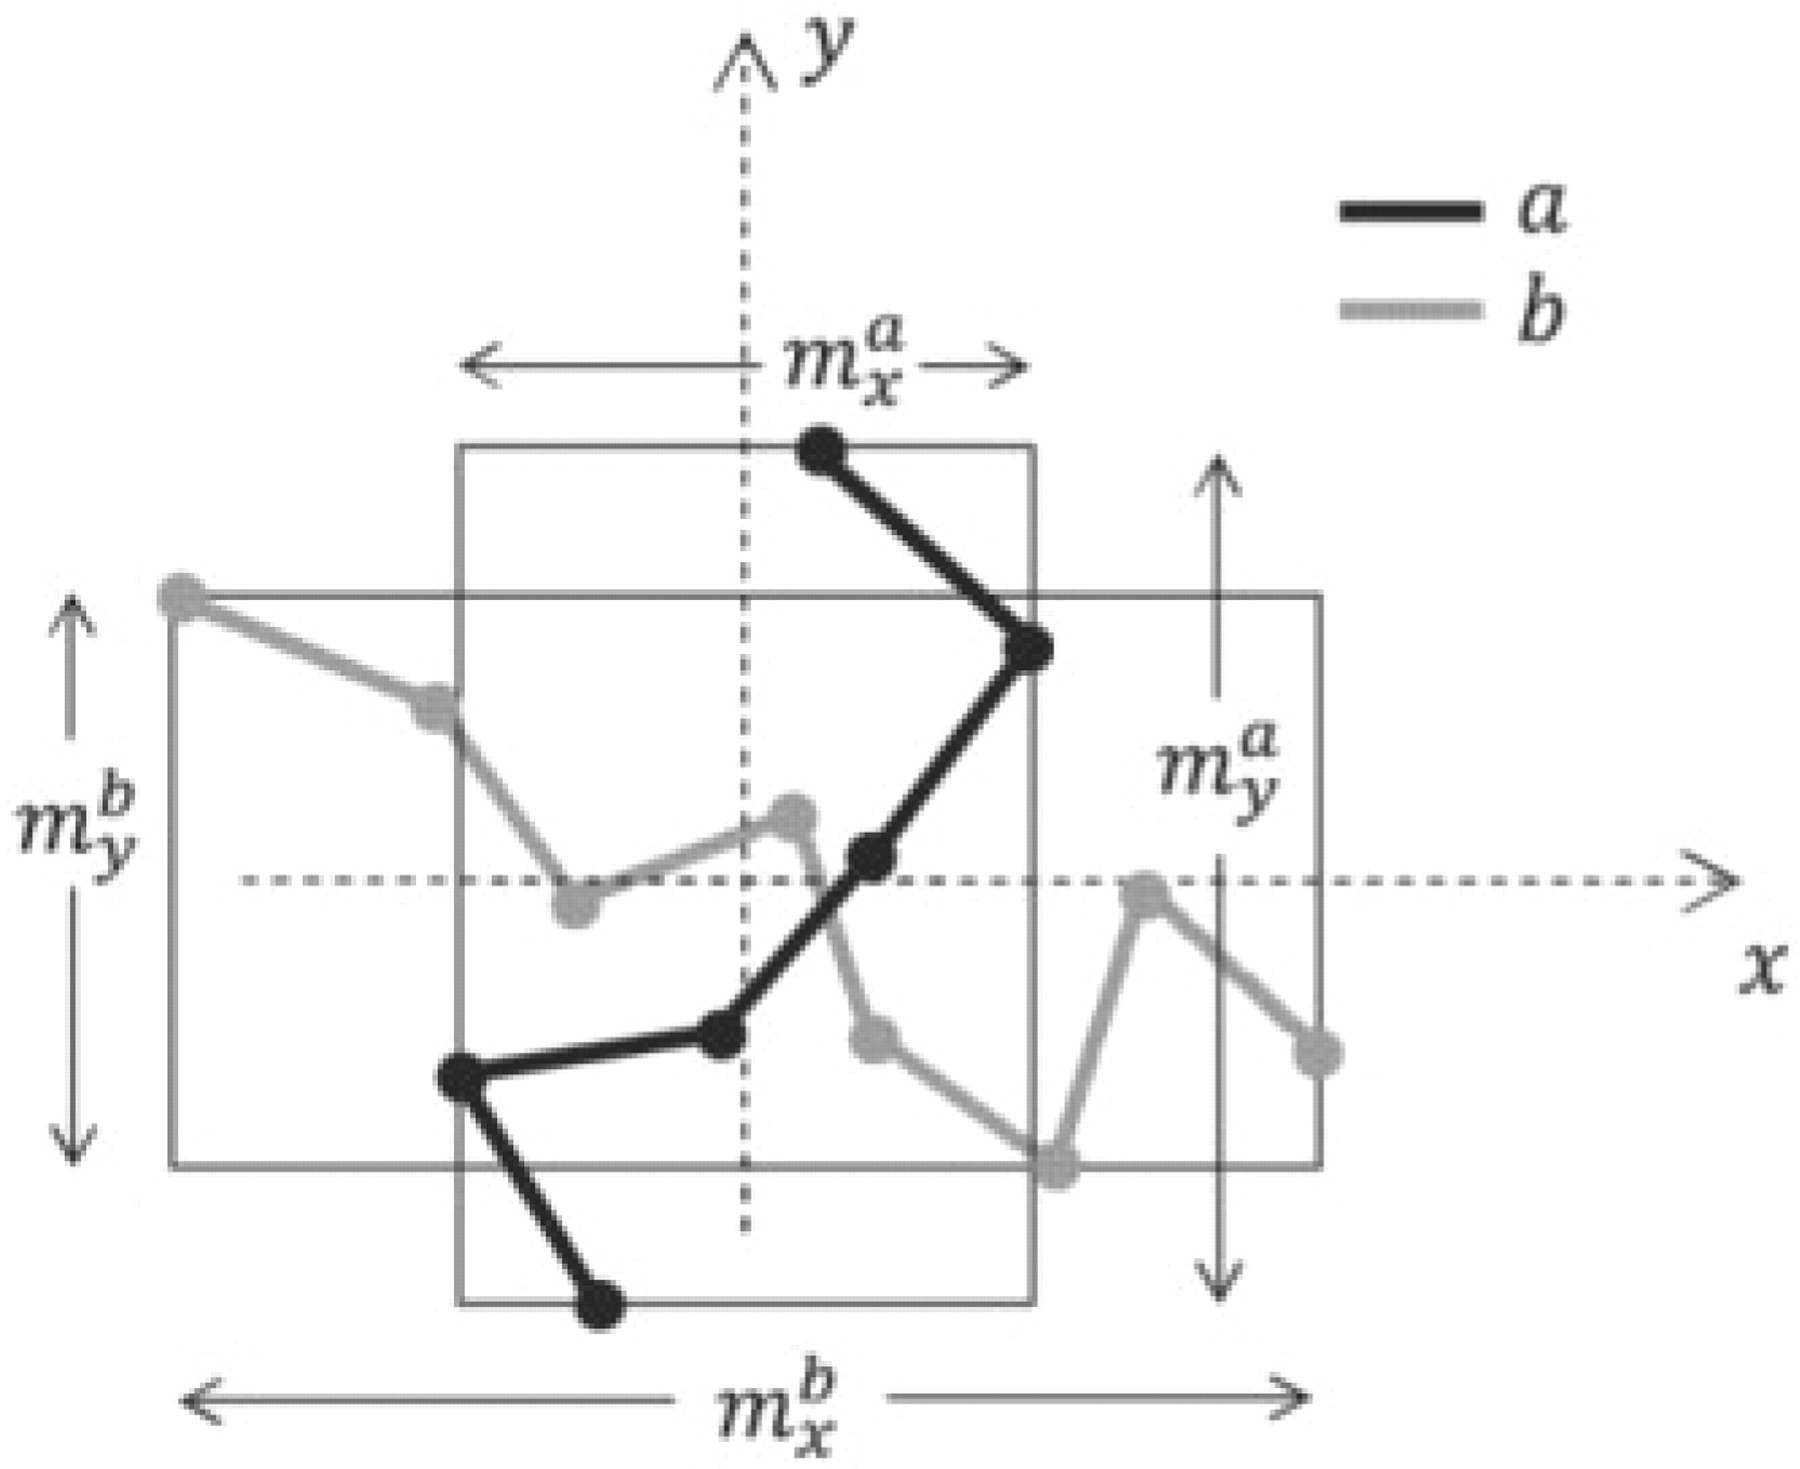
\includegraphics[scale=0.28]{../pictures/btp530f1.jpeg}
\end{figure}

Для дальнейшего уменьшения размера пространства определим конечную $\eps$-сеть преобразований из интервала $I$, полученную разбиением на небольшие шестимерные ячейки. Точки $\eps$-сети являются вершинами этих ячеек.
\begin{gather}
d_1 = d_2 = d_3 = \frac{\eps}{3\sqrt{2}R_b}\\
d_4 = d_5 = d_6 = \frac{\eps}{\sqrt{3}}
\end{gather}

Заметим, что для нахождения $t_\eps^\sigma$ достаточно проверить преобразования из $\eps$-сети. Это происходит потому, что для каждого $t=(\alpha, \beta, \gamma, u, v, w) \in I$, существует такая формула преобразования, что:
\begin{gather}
|\alpha - \overline{\alpha}| \leq \frac{d_1}{2}, |\beta - \overline{\beta}| \leq \frac{d_2}{2}, |\gamma - \overline{\gamma}| \leq \frac{d_3}{2}\\
|u - \overline{u}| \leq \frac{d_4}{2}, |v - \overline{v}| \leq \frac{d_5}{2}, |w - \overline{w}| \leq \frac{d_6}{2}
\end{gather}
и следовательно
\begin{gather}
\| t(b_i) - \overline{t}(b_i)\| \leq \eps, \forall b_i \in b
\end{gather}
где $\| t(b_i) - \overline{t}(b_i)\| $ обозначает Евклидово расстояние между $t(b_i)$ и $\overline{t}(b_i)$. В частности, если $t$ -- это $\sigma$-оптимальное преобразование $t^\sigma$, тогда $\overline{t}$ -- это $(\sigma, \eps)$-оптимальное преобразование $t_\eps^\sigma$.

Докажем это утверждение:
\begin{gather*}
\triangleright\\
\| t(b_i) - \overline{t}(b_i)\| = \| t_{tr}(t_{rot}(b_i)) - \overline{t_{tr}}(\overline{t_{rot}}(b_i)) \| = \\ =
\| t_{tr}(t_{rot}(b_i)) - t_{tr}(\overline{t_{rot}}(b_i)) + t_{tr}(\overline{t_{rot}}(b_i)) - \overline{t_{tr}}(\overline{t_{rot}}(b_i)) \| \leq \\ 
\leq
\| t_{tr}(t_{rot}(b_i)) - t_{tr}(\overline{t_{rot}}(b_i))\| + \| t_{tr}(\overline{t_{rot}}(b_i)) - \overline{t_{tr}}(\overline{t_{rot}}(b_i)) \| = \\ =
\| t_{rot}(b_i) - \overline{t_{rot}}(b_i)\| + \| \overline{t_{rot}}(b_i) -\overline{t_{rot}}(b_i) \| \leq \\ \leq
\sqrt{2}R_b(|\alpha - \overline{\alpha}| + |\beta - \overline{\beta}| + |\gamma - \overline{\gamma}|) + \sqrt{(u - \overline{u})^2 + (v - \overline(v))^2 + (w - \overline{w})^2} \leq \\ \leq
\sqrt{2}R_b \lp \frac{d_1}{2} + \frac{d_2}{2} + \frac{d_3}{2} \rp + \sqrt{\frac{d_4^2}{4} + \frac{d_5^2}{4} + \frac{d_6^2}{4}} = \eps\\
\triangleleft\\
\end{gather*}

Псевдокод данного алгоритма:
\begin{algorithmic}[1]
\item Перенесём центры масс белков $a$ и $b$ в начало координат.
\item Вычислим $M_x, M_y, M_z, R_b$.
\item $r_{\alpha, \gamma} \la \ls \frac{6\sqrt{2}\pi R_b}{\eps}\rs$
\item $r_{\beta} \la \ls \frac{3\sqrt{2}\pi R_b}{\eps}\rs$
\item $s_x \la \ls 1 + \frac{2\sqrt{3}M_x}{\eps} \rs$
\item $s_y \la \ls 1 + \frac{2\sqrt{3}M_y}{\eps} \rs$
\item $s_z \la \ls 1 + \frac{2\sqrt{3}M_z}{\eps} \rs$
\item $d_r \la \frac{\eps}{3\sqrt{2}R_b}$
\item $d_t \la \frac{\eps}{\sqrt{3}}$
\item $bestScore \la 0$
\For{$0 \leq i_1 \leq r_{\alpha, \gamma}, 0 \leq i_2 \leq r_{\beta}, 0 \leq i_3 \leq r_{\alpha, \gamma}$}
\For{$0 \leq i_4 \leq s_x, 0 \leq i_5 \leq s_y, 0 \leq i_6 \leq s_z$}
\State $t \la (i_1d_r, i_2d_r, i_3d_r, -M_x + i_4d_t, -M_y + i_5d_t, -M_z + i_6d_t)$
\If {$|S(a, t(b), \sigma + \eps)| > bestScore$}
    \State $bestScore \la |S(a, t(b), \sigma + \eps)|$
    \State $t_{best} \la t$
\EndIf
\EndFor
\EndFor
\State \Return $t_{best}$
\end{algorithmic}
\section{Время работы}

Для пары белков длины $n$, худший слушай работы данного алгоритма происходит, когда радиус ограничивающей сферы белка $b$ линеен относительно $n$, то есть $R_b = O(n)$. В этом случае общее число преобразований, проверенных данным алгоритмом, равно $\mathbf{NET}(\eps) = O \lp \frac{n^6}{\eps^6} \rp$. Для каждого такого преобразования оптимальное соответствие может быть вычислено с использованием процедуры динамического программирования $O(n^2)$, что приводит к наихудшему времени работы $O \lp \frac{n^8}{\epsilon^6} \rp$.
Однако общая стоимость данного алгоритма, как правило, лучше на практике, так как объём белка пропорционально масштабируется с количество остатков. Например, если $b$ -- глобулярный белок, тогда $R_b = O(n^\frac{1}{3})$, и таким образом время работы данного алгоритма равно только $O\lp\frac{n^4}{\eps^6}\rp$.
Для сравнения алгоритм Колодного и Линеала для оптимизации класса оценочных функций, удовлетворяющих условию Липшица, равна $O \lp \frac{n^{10}}{\eps^6} \rp$ для глобулярных и $O \lp \frac{n^{12}}{\eps^6} \rp$ для неглобулярных белков.

\section{ Качество решения}

Качество решения $t_\eps^\sigma$ представленного $\eps$-оптимальным алгоритмом определяется как разность между оценкой оптимального решения $t^\sigma$ и оценкой $t_\eps^\sigma$:
\begin{gather}
Err(t_\eps^\sigma ) = |S(a, t^\sigma (b), \sigma) | - (S(a, t_\eps^\sigma (b), \sigma)|
\end{gather}

Пока $Err(t_\eps^\sigma)$ не может вычислен в пределах временного окна $\eps$-оптимального алгоритма (так как не известен $t^\sigma$), верхняя граница $Err(t_\eps^\sigma)$:
\begin{gather}
MaxErr(t_\eps^\sigma ) = |S(a, t_\eps^\sigma (b), \sigma + \eps)| - |S(a, t_\eps^\sigma(b), \sigma)|
\end{gather}

Данное выражение может вычислено за счёт маленькой модификации $\eps$-оптимального алгоритма, без увеличения асимптотической сложности.

\section{Оптимальное решение}

Процедура нахождения оптимального решения базируется на том наблюдении, что $f(\sigma) = |S(a, t^\sigma (b), \sigma)|$ это функция, которую можно разбить на некоторое конечное число значений $\sigma_1, \dots, \sigma_k$. Если $\sigma > 0$ -- некоторое действительное число отличное от $\sigma_i, \forall i \in [1, k]$, тогда для достаточно малого $\eps > 0$ получаем $f(\sigma + \eps) = f(\sigma - \eps)$.    

\begin{gather*}
f(\sigma + \eps) = |S(a, t^{\sigma + \eps}, \sigma + \eps)| \geq |S(a, t_\eps^\sigma (b), \sigma + \eps)| \geq\\ \geq
|S(a, t^\sigma (b), \sigma)| \geq |S(a, t^{\sigma - \eps}_\eps (b), \sigma)| \geq \\ \geq
|S(a, t^{\sigma - \eps (b)}, \sigma - \eps)| = f(\sigma - \eps)
\end{gather*}

Отсюда следует, что для каждого такого $\eps$ существует преобразование $t_\eps^{\sigma - \eps}$, которое является оптимальным.

\begin{figure}
\caption{}
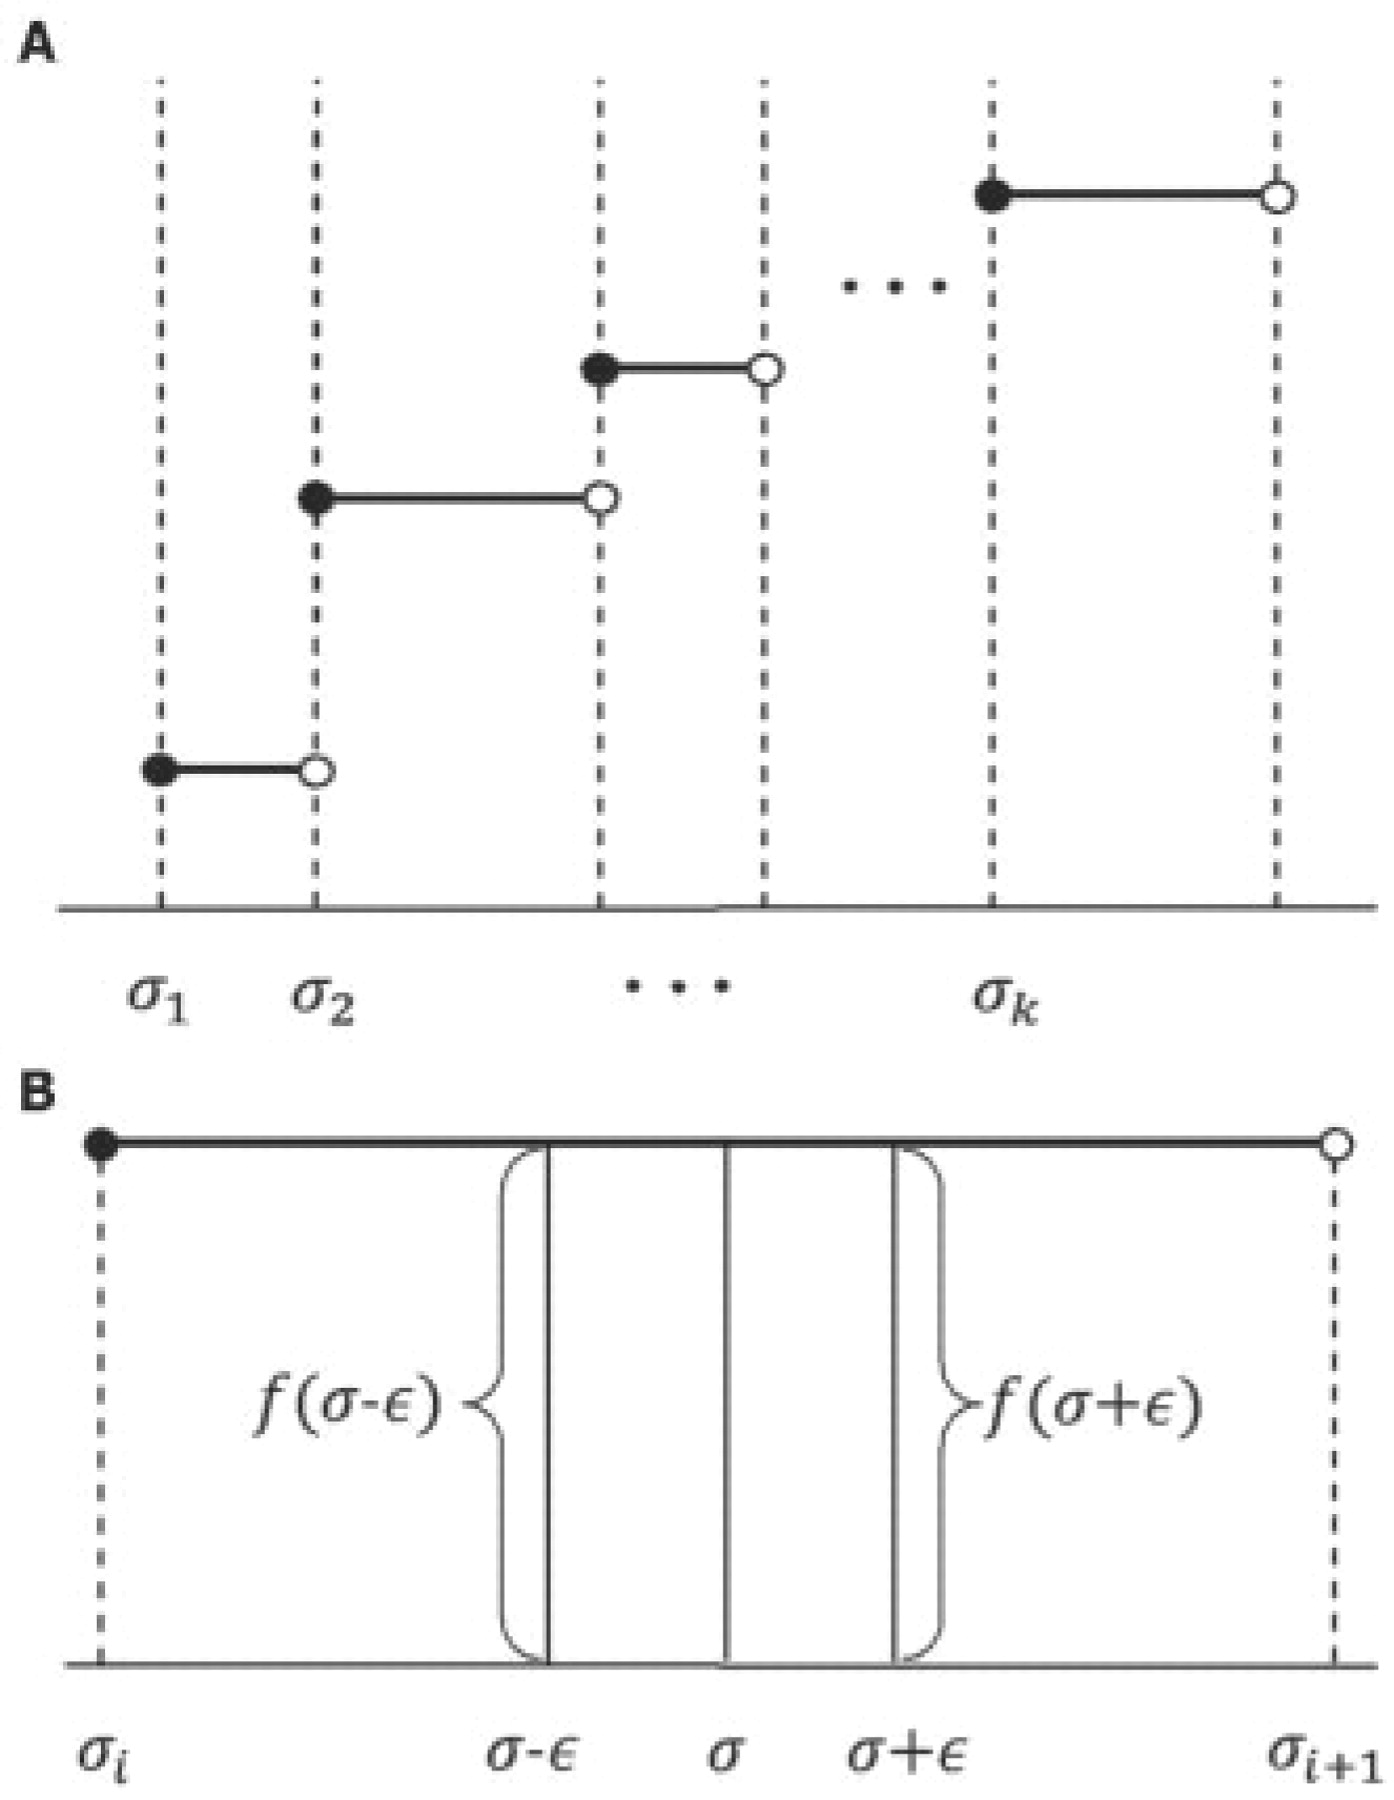
\includegraphics[scale=0.34]{../pictures/btp530f2.jpeg}
\end{figure}

Опишем полученный алгоритм в виде псевдокода.

OPTIMAL($a, b, \sigma$). Отметим, что OPTIMAL возвращает оптимальное решение с вероятностью 1, то есть в случаях, когда $\sigma$ не совпадает ни с одним из фиксированных значений $\sigma_1, \dots, \sigma_k$. Однако число операций, выполненных OPTIMAL, нельзя оценить заранее, так как время её выполнения зависит от разности между $\sigma$ и ближайшим $\sigma_i$ (которая зависит от внутренней геометрии входных белков $a$ и $b$). 

\begin{algorithmic}[1]
\State $\eps \la 1$
\State $t_\eps^\sigma \la \mathrm{EPSILON-OPTIMAL}(a, b, \sigma, \eps)$
\State $t_eps^{\sigma - \eps} \la \mathrm{EPSILON-OPTIMAL}(a, b, \sigma - \eps, \eps)$
\State $\eps \la \frac{\eps}{2}$
\While{$|S(a, t_\eps^\sigma (b), \sigma + \eps )| - |S(a, t_\eps^{\sigma - \eps}(b), \sigma ) > 0$}
\State $t_\eps^\sigma \la \mathrm{EPSILON-OPTIMAL}(a, b, \sigma, \eps)$
\State $t_eps^{\sigma - \eps} \la \mathrm{EPSILON-OPTIMAL}(a, b, \sigma - \eps, \eps)$
\State $\eps \la \frac{\eps}{2}$
\EndWhile
\State \Return $t_\eps^{\sigma - \eps}$
\end{algorithmic}

\section{Практическое применение}

Помимо относительно малого времени работы, $\eps$-оптимальный алгоритм поддаётся параллельным вычисления, так как NET ($\eps$) может быть разделена и процедура поиска будет проводиться одновременно на нескольких подмножествах NET($\eps$). Для оценки потенциальных преимуществ параллельных реализаций данного алгоритма была разработана более быстрая эвристическая версия алгоритма называемая MAX-PAIRS.

Для эффективности MAX-PAIRS исследуют только небольшое подмножество NET($\eps$), состоящее только из тех преобразований из NET($\eps$), которые близки к некоторым "начальным" преобразованиям, обладающим высокой оценкой. Предполагается, что оптимальное преобразование находится не далеко от преобразования с достаточно высокой оценкой, полученного некоторым быстрым и достаточно точным эвристическим методом.

Для вычисления каждого начального преобразования MAX-PAIRS применят хорошо известный итеративный алгоритм расширения выравнивания до $S = S(a, t(b), \sigma)$, где $t$-преобразование, минимизирующее RMSD между короткими отрезками k последовательных остатков в $a$ и $b$ (по умолчанию $k = 5$). На каждой итерации алгоритма расширения белки накладываются, чтобы минимизировать RMSD между выровненными остатками, и новое выравнивание вычисляется динамическим программированием. Вся процедура повторяется до тех пор, пока длина $|S(a, t(b)), \sigma)|$ остаётся неизменной между двумя последовательными итерациями.

После генерации всех начальных преобразований с высокой оценкой, MAX-PAIRS "уточняют" их по одному исследую ближайшие трансформации из NET($\eps$). Более конкретно (и предполагая, что начальным трансформации уже применены к $b$), алгоритм выбирает три пары выровненных точек 
\begin{gather*}
\{(a_{i_k}, b_{i_k})\}, k = \overline{1, 3}
\end{gather*} 
из $S(a, b, \sigma)$, а затем ищет NET($\eps$), сохраняя точки $a_{i_k}$ и $b_{i_k}$ связанными, то есть лежащими на расстоянии не более $\sigma$. Изучая только преобразования $\tau$ такие, что $\| a_{i_k} - \tau(b_{i_k})\| \leq \sigma, \forall k \in \{1, 2, 3 \}$. MAX-PAIRS значительно уменьшает размер пространства поиска, что приводит к повышению эффективности.

Опишем процедуру уточнения более подробнее. Без потери общности пологаем, что точка $b_{i_1}$ -- это точка начала координат, точка $b_{i_2}$ -- лежит в положительной части прямой $y$, а точка $b_{i_3}$ лежит на плоскости $yz$.

\begin{figure}
\caption{}
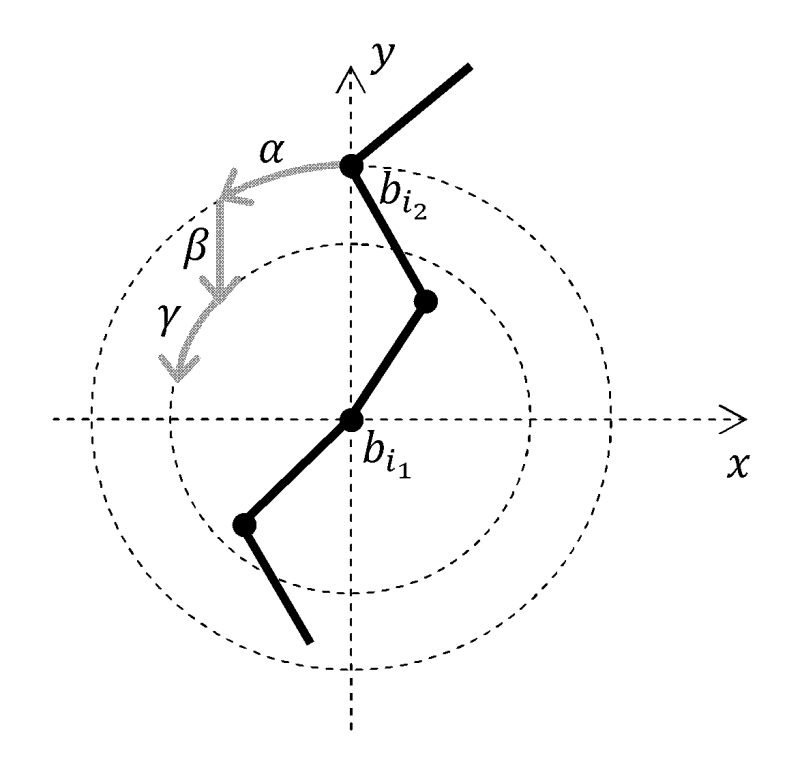
\includegraphics[scale=2]{../pictures/pic1.png}
\end{figure}

Для уменьшения размера пространства поиска, мы можем исключить из него все преобразования $t=(\alpha, \beta, \gamma, u, v, w)$ такие, что $|u| > 2\sigma$, или $|v| > 2\sigma$, или $|w| > 2\sigma$, потому что каждое такое преобразование ломает связь между $a_{i_1}$ и $b_{i_1}$:
\begin{gather*}
\|t(b_{i_1}) - a_{i_1} \| = \|t(b_{i_1}) - b_{i_1} + b_{i_1} - a_{i_1}\| \geq \\ \geq
\| t(b_{i_1}) - b_{i_1}\| - \|b_{i_1} - a_{i_1}\| > 2\sigma - \sigma = \sigma
\end{gather*}

Также можно избавиться от определённых комбинаций углов $\alpha$ и $\gamma$, то есть от преобразований $t = (\alpha, \beta, \gamma, u, v, w)$ таких, что:
\begin{gather*}
\cos (\alpha + \gamma) < 1 - \frac{8\sigma^2}{\|b_{i_2}\|^2}
\end{gather*}
и любой из $\alpha, gamma \in [0, \frac{\pi}{2}] \cup [\frac{3\pi}{2}, 2\pi]$ или $\alpha, \gamma \in [\frac{\pi}{2}, \frac{3\pi}{2}]$. Для всех таких преобразований:
\begin{gather*}
\| t_{rot} (b_{i_2} - b_{i_2} \| = \sqrt{2} \|b_{i_2}\| \sqrt{1 + \sin \alpha \sin\gamma - \cos\alpha\cos\beta\cos\gamma} \geq \\ \geq
\sqrt{2}\|b_{i_2}\| \sqrt{1 - \cos(\alpha + \gamma)} > 4\sigma
\end{gather*} 
и поэтому:
\begin{gather*}
\|t(b_{i_2} - a_{i_2}\| = \|t_{rot}(b_{i_2} - b_{i_2} + t_{tr}(t_{rot}(b_{i_2})) - t_{rot}(b_{i_2}) + b_{i_2} - a_{i_2} \| \geq \\ \geq
 \|t_{rot} (b_{i_2}) - b_{i_2} \| - \| t_{tr} (t_{rot}(b_{i_2})) - t_{rot} (b_{i_2}) \| - \| b_{i_2} - a_{i_2} \| > \\ > 
 4\sigma - 2\sigma - \sigma = \sigma
\end{gather*}
(полагается, что пространство было уменьшено до преобразований удовлетворяющих условию $\|t_{tr}(t_{rot}(b_{i_2})) - t_{rot}(b_{i_2})\| < 2\sigma$).

Аналогичная аргументация может быть использована чтобы показать, что если $\alpha \in [0, \frac{\pi}{2}] \cup [\frac{3\pi}{2}, 2\pi]$ и $\gamma \in [\frac{\pi}{2}, \frac{3\pi}{2}]$, или наоборот, то можно уменьшить пространство преобразований удалив преобразования $t = (\alpha, \beta, \gamma, u, v, w)$, такие что:
\begin{gather*}
\cos(\alpha - \gamma) > \frac{8\sigma^2}{\|b_{i_2}\|^2} - 1
\end{gather*}

Для того, чтобы уменьшить пространство преобразований ещё больше, отметим, что если $r$ -- это точка на оси $z$ такая что $\\r\| = \|b_{i_3}\|$, тогда каждое преобразование удовлетворяющее следующему неравенству:
\begin{gather*}
\cos\beta < 1 - \frac{2(2\sigma + d)^2}{\|b_{i_3}\|^2}
\end{gather*}
ломает связь между $a_{i_3}$ и $b_{i_3}$, где $d=\|r-b_{i_3}\|$.

\begin{figure}
\caption{}
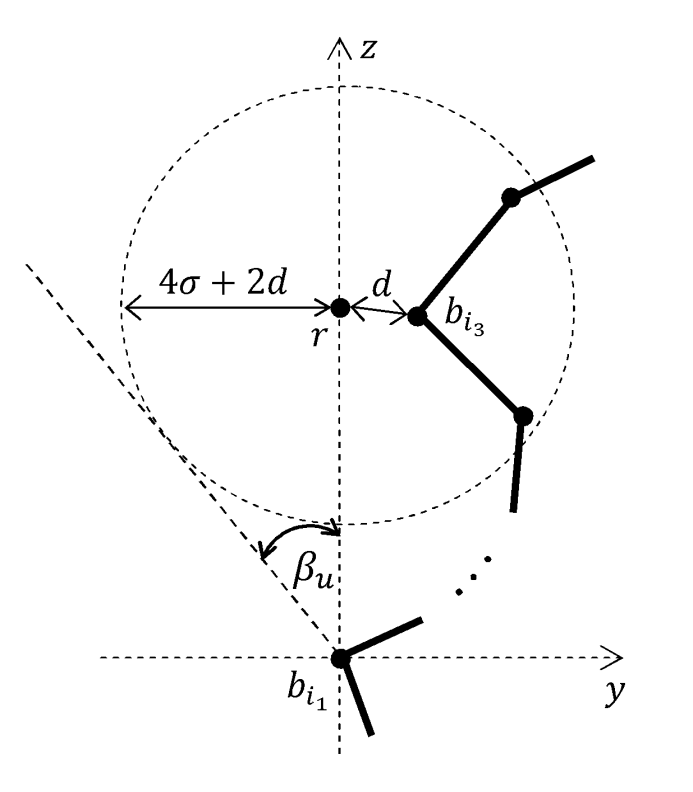
\includegraphics[scale=1.9]{../pictures/pic2.png}
\end{figure}

И, наконец, не сложно заметить, что наилучшее уменьшение пространства преобразований достигается, когда выбираются точки $\{b_{i_k}\}_{k = 1}^3$ так, чтобы максимизировать $\|b_{i_2}\|$ и $\|b_{i_3}\|$, а также минимизировать $d$.

\section{ Результаты работы}

Производительность MAX-PAIRS была протестирована на репрезентативном наборе белковых цепочек, отобранных из базы данных SCOP. Набор для тестирования содержит 195 пар белков связанных на различных условиях согласно структурной классификации SCOP: 57 family пар, 75 superfamily пар, и 63 fold-пары.

Для эффектиности параметр точности $\eps$ MAX-PAIRS устанавливается равным 1 (уменьшение $\eps$ даёт более точную, но менее эффективную процедуру). Оценки для MAMMOTH и MUSTANG, представленные в таблицах, показаны только для справки, так как в отличие от MAX-PAIRS и LGA, которые максимизируют функцию $CA \leq \sigma$, эти программы стремятся оптимизировать другую целевую функцию.

\begin{table}
\caption{ Общее число пар в тестовом наборе, которые могут быть наложены на расстояние не превосходящем 3 \angstrom}
\begin{center}
\begin{tabular}{|c|ccccc|}
\hline
& MAX-PAIRS & LGA & TM-alogn & Mammoth & Mustang\\
\hline
Family & 4689 & 4585 & 4460 & 4264 & 4231\\
Superfamily & 4378 & 4247 & 4140 & 3713 & 3319\\
Flod & 2870 & 2720 & 2634 & 2100 & 1834\\
\hline
\end{tabular}
\end{center}
\end{table}

\begin{table}
\caption{ Общее число пар в тестовом наборе, которые могут быть наложены на расстояние не превосходящем 5 \angstrom}
\begin{center}
\begin{tabular}{|c|ccccc|}
\hline
& MAX-PAIRS & LGA & TM-alogn & Mammoth & Mustang\\
\hline
Family & 5261 & 5130 & 5059 & 5019 & 4983\\
Superfamily & 5240 & 5033 & 4928 & 4702 & 4532\\
Flod & 3575 & 3409 & 3279 & 2842 & 2816\\
\hline
\end{tabular}
\end{center}
\end{table}

Как видно из таблиц 1 и 2, даже с $\eps=1$ MAX-PAIRS лучше, по сравнению с другими методами, показываем себя на всех категориях SCOP на обоих расстояних (3\angstrom и 5\angstrom)

На следующем графике можно увидеть распределение добавленного значения MAX-PAIRS, измерено дополнительное число $CA \leq \sigma$ обнаруженных данным алгоритмом. Как видно из левых хвостов на графиках, на некоторых парах белков MAX-PAIRS работает хуже, чем LGA и TM-align. Это не удивительно так как все эти алгоритмы использует различные наборы преобразований для поиска лучшей суперпозиции.

\begin{figure}
\caption{}
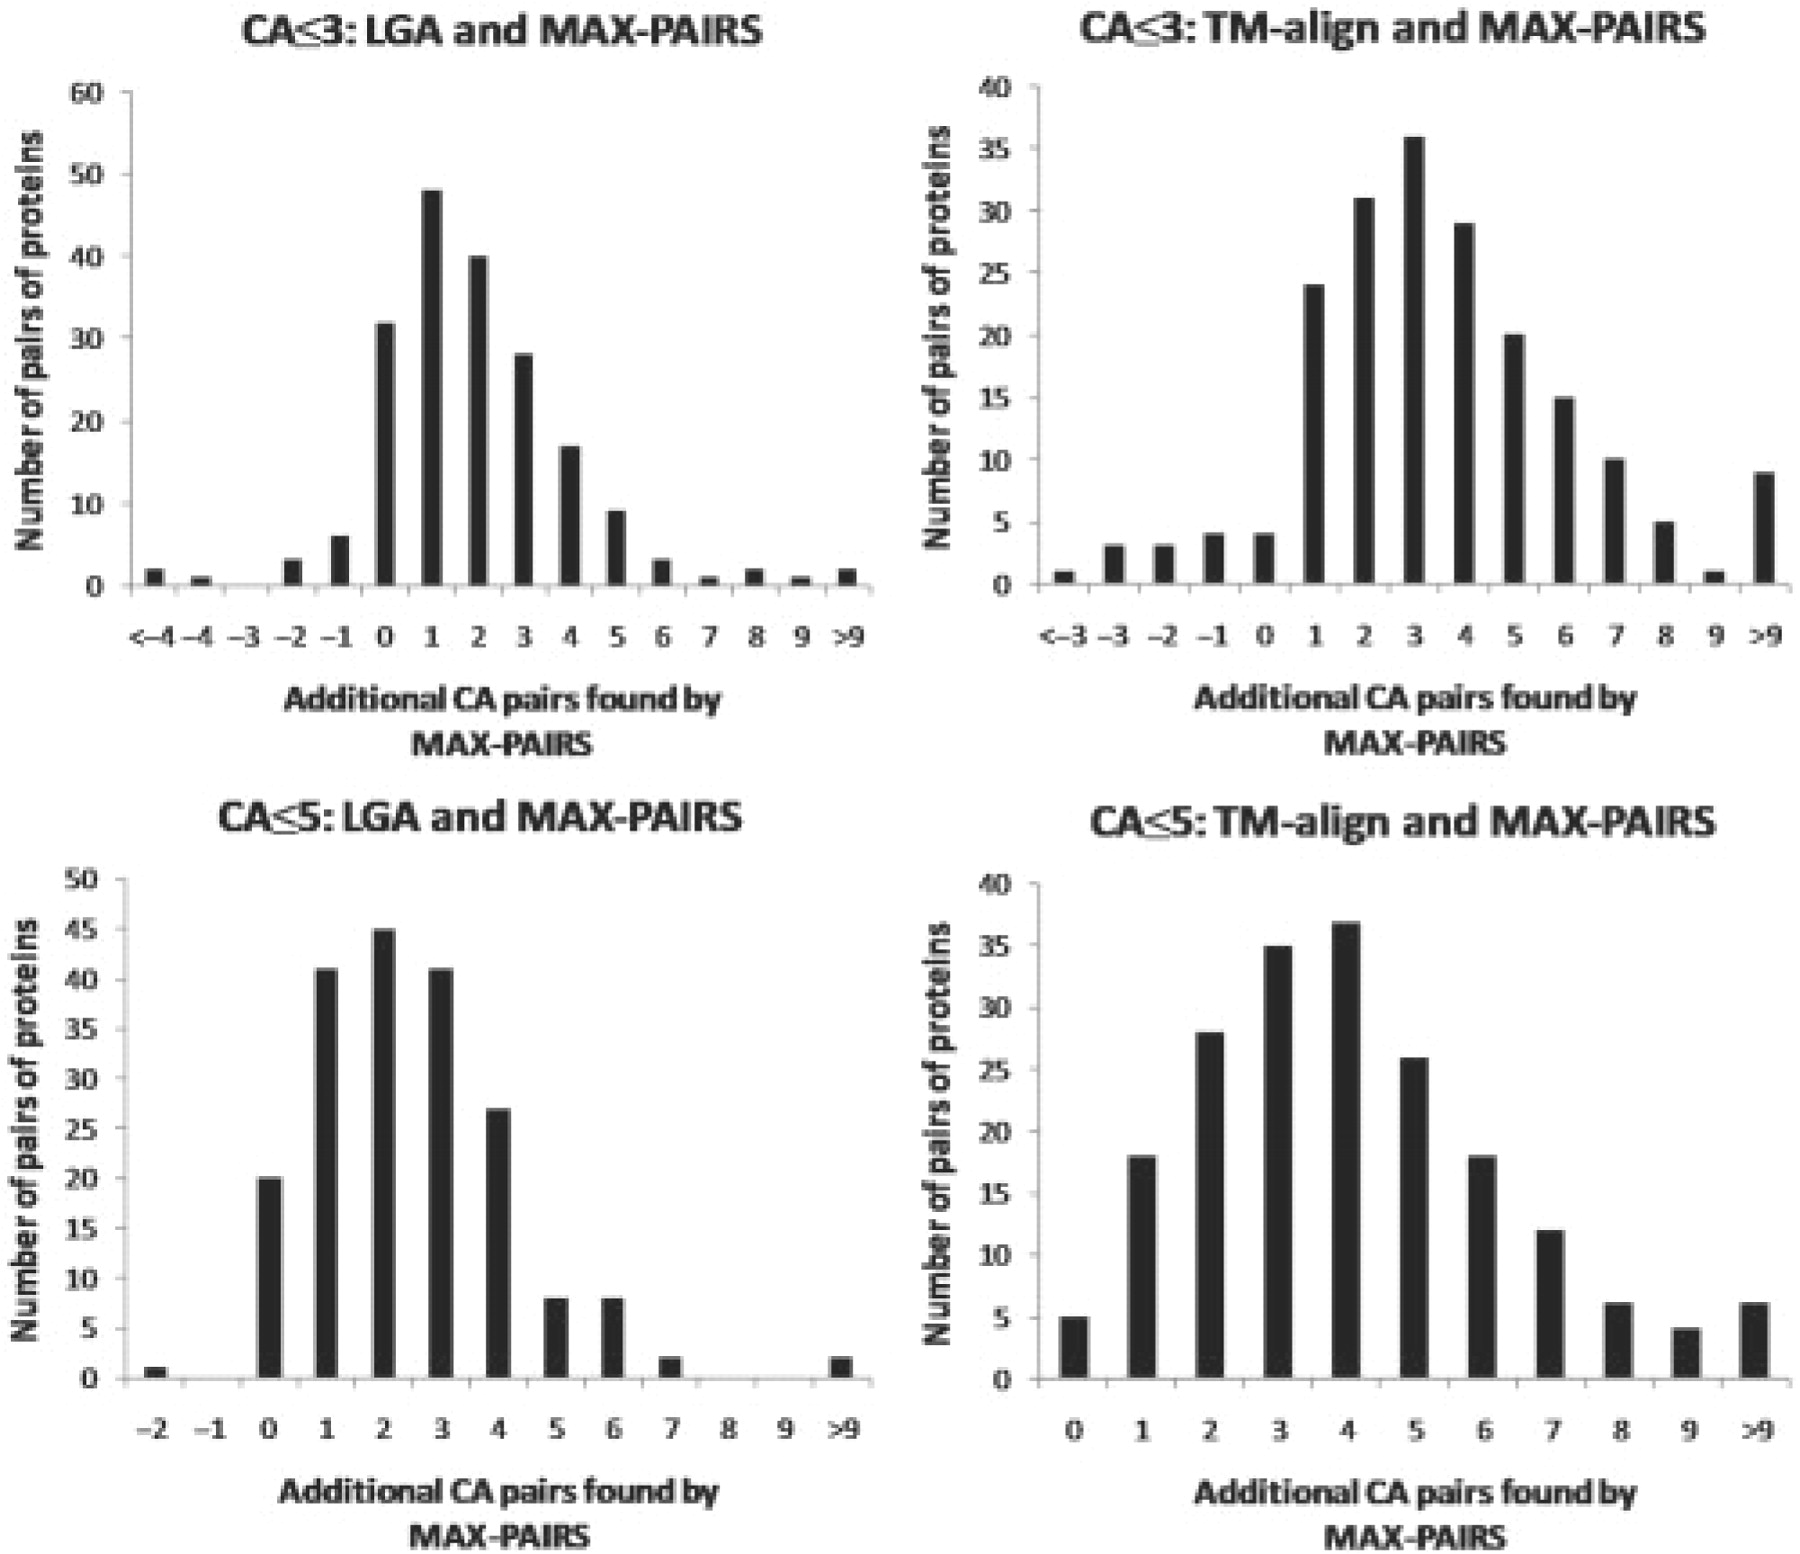
\includegraphics[scale=0.27]{../pictures/btp530f3.jpeg}
\end{figure}

\begin{figure}
\caption{}
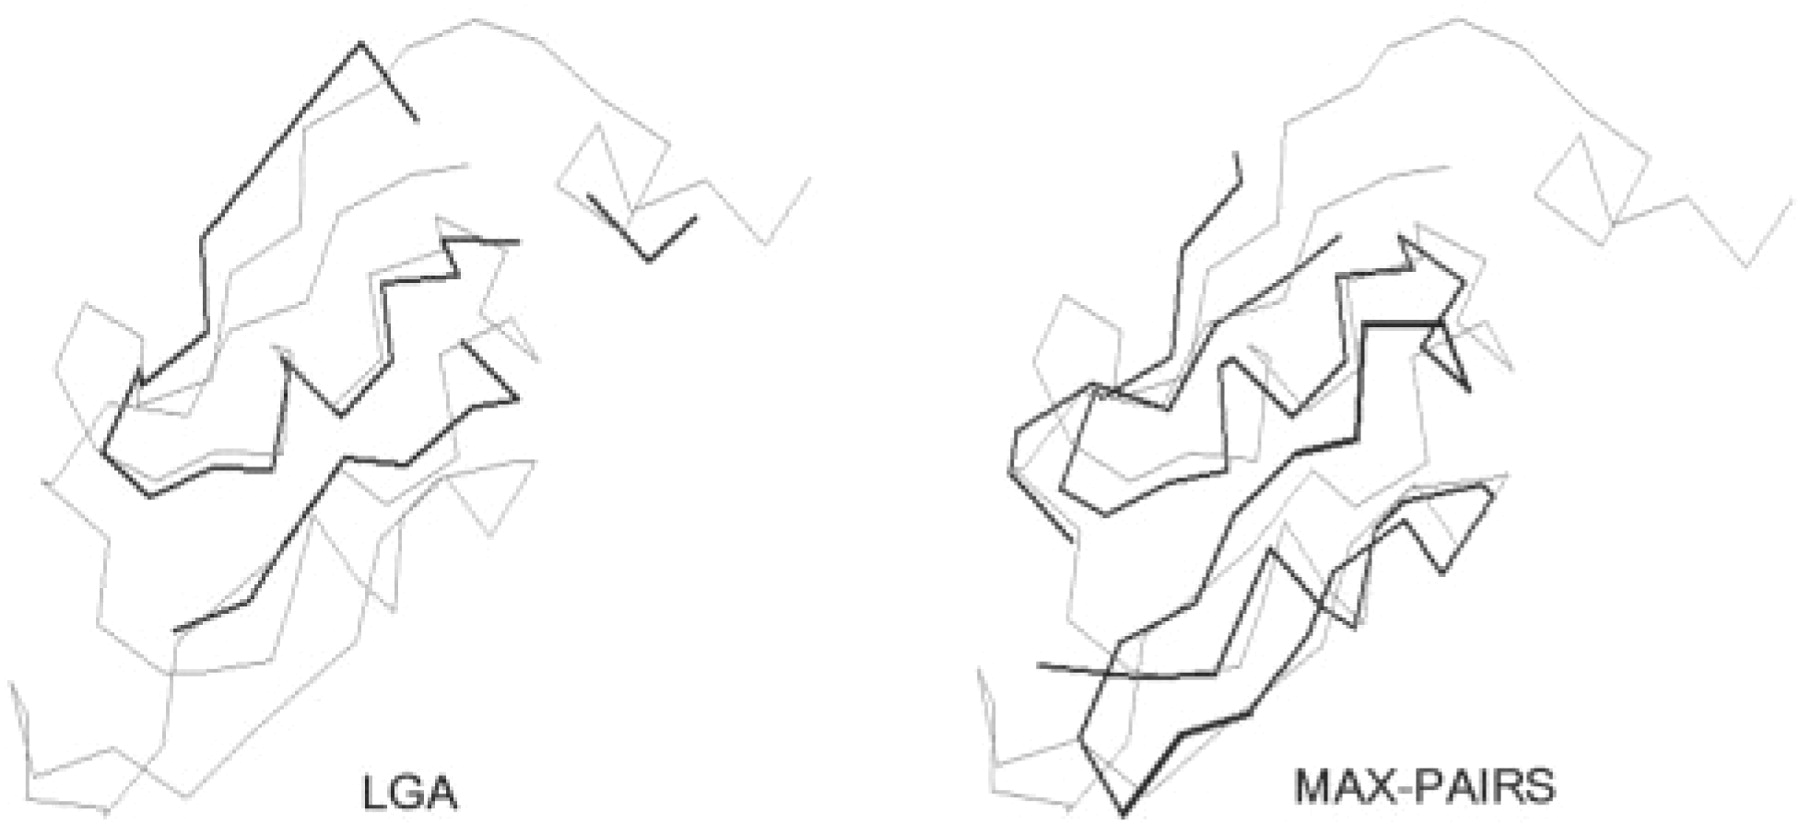
\includegraphics[scale=0.27]{../pictures/btp530f4.jpeg}
\end{figure}

В таблице 3 покажем эффективность MAX-PAIRS как функции зависящей от $\eps$ она множестве пар структур из описанного выше датасета. Анализ был произведён на компьюетере с Intel CPU производительностью 2.2 GHz с операционной системой Linux. Результаты собранные в данной таблице предполагают что, хотя LGA и TM-align намного более эффективные программы по сравнению с MAX-PAIRS однако точность MAX-PAIRS превосходит точности этих алгоритмов для всех протестированных значений $\eps$.

\begin{table}
\caption{ Время работы в зависимости от $\eps$}
\begin{center}
\begin{tabular}{|c|c|c|}
\hline
$\eps$ & $CA \leq 3$  & Время работы одной пары (секунд)\\
\hline
1.0 & 11937 & 6608\\
1.5 & 11862 & 713\\
2.0 & 11789 & 140\\
2.5 & 11711 & 46\\
3.0 & 11602 & 19\\
3.5 & 11566 & 9\\
\hline
\end{tabular}
\end{center}
\end{table}

Многие методы попарного структурного выравнивания белков, включая методы, обсуждаемые в этой работе, используют ключевую процедуру для вычисления суперпозиций, которая максимизирует $CA \leq \sigma$ между парой белковых структур. Вполне разумно ожидать, что улучшение этой суперпозиции повышает точность выравнивания структуры белка. Для оценки степени этого улучшения, используется Sisyphus бенчмарк для точности выравнивания Набор тестов Sisyphus содержит 125 созданных вручную структурных выравниваний для пар белков с нетривиальным структурными отношениями. Эти выравнивания могут быть использованы (как золотые стандарты) для оценки точности метода выравнивания структуры белка. Для того, чтобы сравнить точность выравнивания алгоритмов в данной работе с точностью методов , ранее протестированных в Sisyphus бенчмарке, использовались только подмножество набора теста Sisyphus содержащего 106 одиночных цепных белков.

Чтобы проверить полезность алгоритмов оптимизации $CA \leq \sigma$, мы модифицировали метод TM-align, заменив исходные суперпозиции TM-align суперпозициями, порождёнными программой MAX-PAIRS. Модифицированная TM-align, названная MP-TM-align, использует TM-align функцию оценивания (TM-score) для вычисления оптимального структурного выравнивания белков совмещённых MAX-PAIRS программой. Как видно из таблицы 4, не только программа MP-TM-align превосходит исходный метод TM-align для каждого сдвига допуска, но и точность этого простого гибридного метода сопоставима с точностью методов проверенных Rocha и коллегами.
\begin{table}
\caption{ Согласование с эталонными выравниваниями для 6 различных сдвигов}
\begin{center}
\begin{tabular}{|c|cccccc|}
\hline
&0&1&2&3&4&5\\
\hline
FLEXPROT&               0.449&  0.672&  0.707&  0.725&  0.742&  0.747\\
MATRAS&                 0.776&  0.806&  0.828&  0.836&  0.847&  0.847\\
PD&                             0.791&  0.849&  0.858&  0.868&  0.881&  0.882\\
PPM&                    0.782&  0.813&  0.823&  0.833&  0.843&  0.844\\
RASH&                   0.688&  0.793&  0.812&  0.840&  0.854&  0.855\\
SSAP&                   0.750&  0.786&  0.797&  0.804&  0.808&  0.811\\
VOROLIGN&               0.722&  0.765&  0.790&  0.808&  0.826&  0.830\\
DALI&                   0.800&  0.830&  0.845&  0.851&  0.859&  0.860\\
MATT&                   0.829&  0.866&  0.889&  0.904&  0.915&  0.917\\
LGA&                    0.765&  0.820&  0.831&  0.839&  0.847&  0.849\\
TM-align&               0.762&  0.815&  0.823&  0.834&  0.841&  0.844\\
MP-TM-align&    0.809&  0.861&  0.875&  0.884&  0.896&  0.896\\
MP-TM-align+&   0.830&  0.867&  0.881&  0.887&  0.897&  0.898\\
\hline
\end{tabular}
\end{center}
\end{table}

Интересно отметить, что, согласно исследованию Rocha, наиболее точные методы структурного выравнивания, такие как Matt, PPM и ProtDeform, рассматривают белки, как гибкие объекты. Эти методы достигают высокой точность выравнивания, применяя последовательность различных жёстких преобразований на разных участках, а не одно глобальное жёсткое преобразование. С другой стороны, результаты данного исследования показывают, что всё ещё могут быть разработаны высокоточные методы, которые опираются на одно жёсткое преобразование для оценки сходства белковых структур.

Ещё большее повышение точности TM-align может быть достигнуто за счёт использования информации о типе остатков в процессе выравнивания. Комбинирование мер на основе расстояния с оценками мутации остатков является стандартным методом, используемым во многих методах выравнивания структуры, таких как CE. Как видно из таблицы 4, вариант MP-TM-align метода, названный MP-TM-align+, которое основано на совмещённой функции оценки, определённой как сумма TM-score и BLOSUM62 score даёт самое точное выравнивание согласно Sisyphus benchmark.

При более подробном рассмотрении результатов, обобщённых в таблице 4, и результатов, полученных Rocha и другими, выявлена существенная разница TM-align в этих двух исследованиях. Это различие объясняется тем, что в двух экспериментах использовались разные версии TM-align. Более конкретно, программа TM-align, протестированная в данном тесте, выпущена 14 марта 2009 года и на 4\% более точна, чем старая программа, оценённая в тесте Rocha.

Выравнивание белков в наборе тестов Sisyphus, созданное LGA, TM-align, MP-TM-align и MP-TM-align+ может быть загружено отсюда:\\
\url{http://bioinformatics.cs.uni.edu/opt_align.html}. 

Выравнивание сгенерированное десятью другими методами может быть скачано отсюда:\\ 
\url{http://dmi.uib.es/people/jairo/bio/ProtDeform}.

Также осталось много работы по ускорению MAX-PAIRS, требуется сделать его практичным для крупномасштабного анализа структуры белков. Однако даде в нынешнем видел MAX-PAIRS может быть полезен при оценке эффективности методов прогнозирования структуры белка. Например точность MAX-PAIRS на 3,6\% выше точности программы LGA, официально используемой на двухгодичном конкурсе CASP. Это значительное преимущество метода MAX-PAIRS,учитывая, что разница в баллах GDT\_TS между первым и вторым методами ранжирования в CASP7, измеренная LGA, составляет всего 2.6\% (3.5\% в CASP8).

\addcontentsline{toc}{chapter}{Заключение}
\chapter*{Заключение}

Выводы о подобии двух белков зачастую получают на основе их структурного сходства. Однако из-за бесконечного (несчётного) пространства всех возможных пространственных конфигураций, нахождение суперпозиции для пары белков является очень трудоёмкой задачей.

В этой работе показано, что проблему приближённого структурного выравнивания можно трактовать различными метриками структурного выравнивания, такими как GDT, AL0 и MaxSub. Хотя описанный в данной статье алгоритм для почти оптимального решения потребляет большое вычислительное время, время работы можно легко уменьшить с помощью параллельных реализаций. Дополнительным преимуществом алгоритма для приближённого решения является то, что он обеспечивает меру качества решения, которая сигнализирует, является ли возвращённая суперпозиция, по сути, оптимальной суперпозицией.

Также в данной работе представлена процедура, способная найти оптимальную суперпозицию любых двух белков для всех, кроме конечного числа порогов, расстояний. Однако такая программа для поиска оптимального решения слишком медленная для практического применения.

\newpage
\addcontentsline{toc}{chapter}{Cписок Литературы}

\chapter*{ Список литературы}

\begin{itemize}
\item[1] Andreeva
A
, et al. 
SISYPHUS—structural alignments for proteins with non-trivial relationships
, Nucleic Acids Res.
 , 2007
, vol. 35
 (pg. D253
-D259)
\item[2]Alexandrov
NN
, et al. 
Common spatial arrangements of backbone fragments in homologous and nonhomologous proteins
, J. Mol. Biol.
 , 1992
, vol. 225
 (pg. 5
-9)
\item[3]Caprara
A
, et al. 
1001 optimal PDB structure alignments: integer programming methods for finding the maximumcontact map overlap
, J. Comput. Biol.
 , 2004
, vol. 11
 (pg. 27
-52)
\item[4]Csaba
G
, et al. 
Protein structure alignment considering phenotypic plasticity
, Bioinformatics
 , 2008
, vol. 24
 (pg. i98
-i104)
\item[5]Eidhammer
I
, et al. 
Structure comparison and structure patterns
, J. Comput. Biol.
 , 2000
, vol. 7
 (pg. 685
-716)
\item[6]Fischer
D
, et al. 
CAFASP3: the third critical assessment of fully automated structure prediction methods
, Proteins
 , 2003
, vol. 53
 Suppl. 6
(pg. 503-516)
\item[7] Ginalski
K
, et al. 
Practical lessons from protein structure prediction
, Nucleic Acids Res.
 , 2005
, vol. 33
 (pg. 1874
-1891)
\item[8] Goldman
D
, et al. 
Algorithmic aspects of protein structure similarity
, Proceedings of the 40th Annual Symposium on Foundations of Computer Science
 , 1999
Washington, DC, USA
IEEE Computer Science
(pg. 512
-522)
\item[9] Goldsmith-Fischman
S
,  Honig
B
. 
Structural genomics: computational methods for structure analysis
, Prot. Sci.
 , 2003
, vol. 12
 (pg. 1813
-1821)
\item[10]Henikoff
S
,  Henikoff
JG
. 
Amino acid substitution matrices from protein blocks
, Proc. Natl Acad. Sci. USA
 , 1992
, vol. 89
 (pg. 10915
-10919)
\item[11]Hao
MH
, et al. 
Effects of compact volume and chain stiffness on the conformations of native proteins
, Proc. Natl Acad. Sci. USA
 , 1992
, vol. 89
 (pg. 6614
-6618)
\item[12] Holm
L
,  Sander
C
. 
Protein structure comparison by alignment of distance matrices
, J. Mol. Biol.
 , 1993
, vol. 233
 (pg. 123
-138)
\item[13]Kabsch
W
. 
solution for the best rotation to relate two sets of vectors
, Acta Crystallographica
 , 1976
, vol. 32
 (pg. 922
-923)
\item[14] Kolodny
R
,  Linial
N
. 
Approximate protein structural alignment in polynomial time
, Proc. Natl Acad. Sci. USA
 , 2003
, vol. 101
 (pg. 12201
-12206)
\end{itemize}
\end{document}
